\subsection{Présentation du club}
\label{subsec:pres_club}

Créée il y a plus de trente ans, AéroIPSA est une des associations aérospatiales de l’école d’ingénieurs \acrshort{IPSA}. Elle a
pour mission de concevoir, développer et mettre en œuvre des projets techniques dans le domaine de l’astromodélisme et du
spatial. Les activités de l’association couvrent l’ensemble du cycle de réalisation, de la conception mécanique et électronique
à la fabrication et aux essais, autour de projets tels que des \gls{Minif}, des \gls{Fusex}, des \glspl{Cansat} ou des systèmes
embarqués. Ces projets constituent un cadre d’application concret des enseignements de l’école et offrent aux étudiants une
première expérience de gestion technique, humaine et opérationnelle.\cite{AeroIPSA}\\

AéroIPSA s’attache également à favoriser la transmission des connaissances entre promotions et la montée en compétences de ses
membres à travers un encadrement technique, des formations internes et des travaux collaboratifs. Chaque année, ces efforts se
concrétisent par la participation de l’association à la campagne nationale de lancements du \gls{C'Space}, organisée par le
\acrshort{CNES} et l'association \gls{Planète Sciences}, où les étudiants valident et présentent les projets réalisés.
\cite{AeroIPSA}

\vfill

\begin{figure}[h]
    \centering
    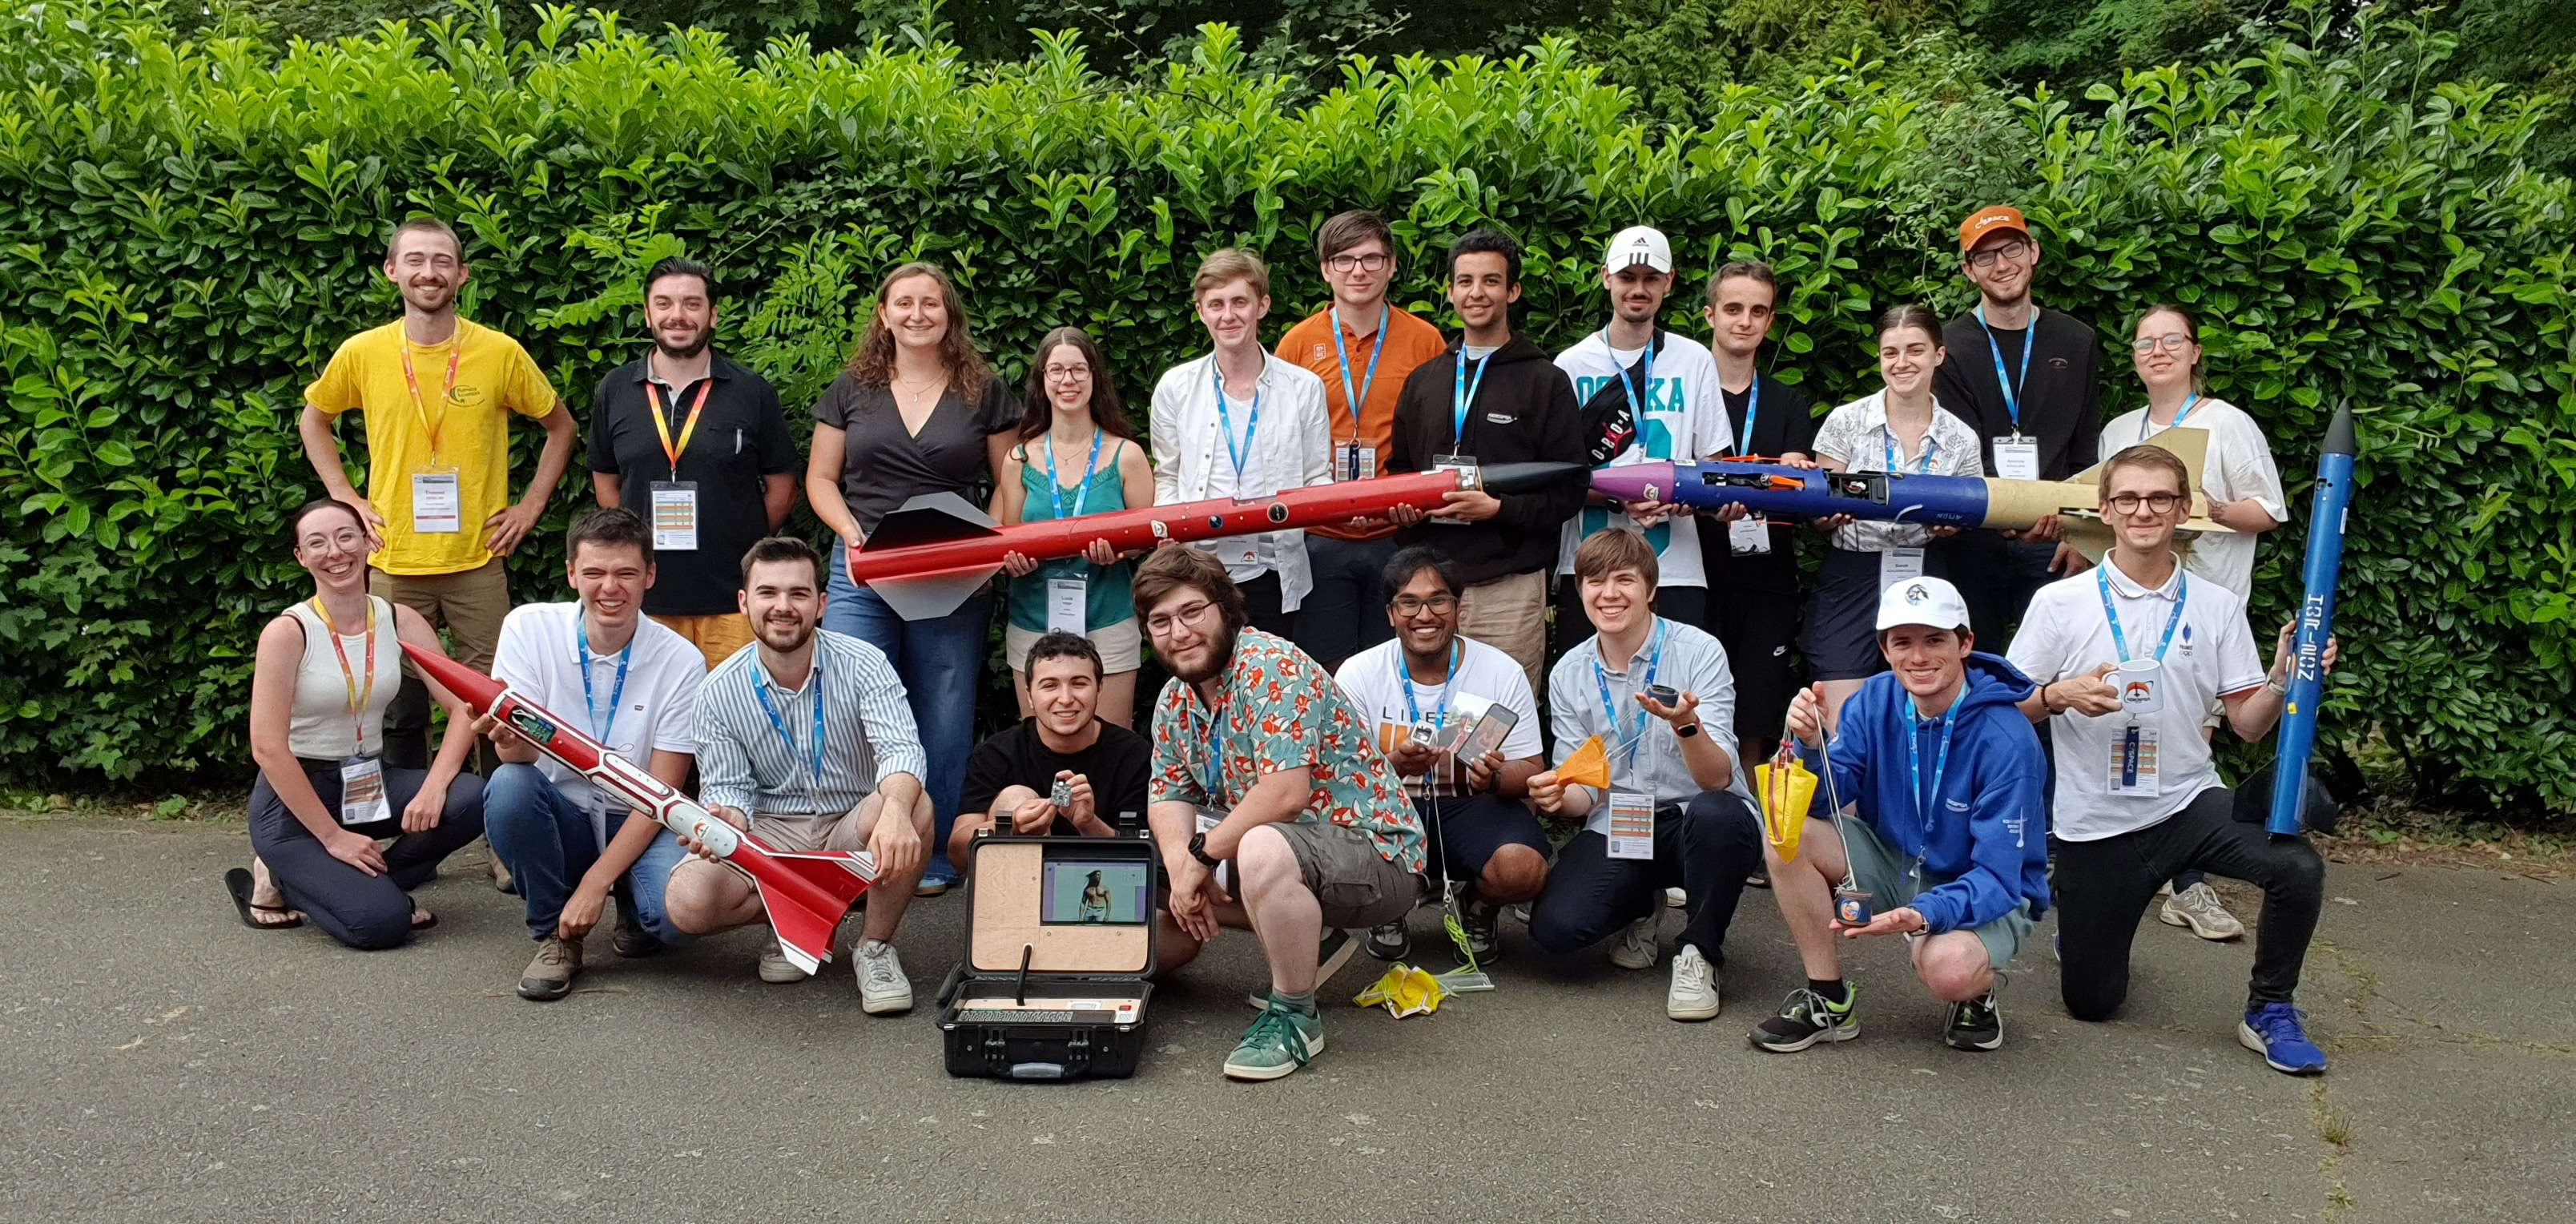
\includegraphics[width=\textwidth]{figures/cspace2025.jpg}
    \caption{Photo de groupe de membre du club de l'AéroIPSA lors du \gls{C'Space} 2025.}
    \label{fig:pres_club}
\end{figure}

\vfill

\newpage
